% mn2eguide.tex
% v2.1 released 03/05/2002
%
% Adapted from mnguide.tex
% v1.3 released 14th September 1995
% v1.2 released 5th September 1994 (M. Reed)
% v1.1 released 18th July 1994
% v1.0 released 28th January 1994


% The journal style files and macros, with guides on their use, are
% available by anonymous FTP on the Internet from the Comprehensive
% TeX Archive Network (CTAN) sites ftp.tex.ac.uk and ftp.dante.de.
% The files are in the directories
% /tex-archive/macros/plain/contrib/mnras and
% /tex-archive/macros/latex209/contrib/mnras for the TeX and LaTeX
% files respectively.



\documentclass[useAMS,usenatbib]{mn2e}

\usepackage{rotating}
\usepackage{lscape}
\usepackage{graphicx}
\usepackage{amssymb}
\usepackage{amsmath}
\usepackage{epstopdf}
\usepackage{color}
\usepackage{soul}
\usepackage{multirow}
\usepackage{longtable}
\usepackage{textcomp}
\usepackage[caption=false]{subfig}
\usepackage{float}
\usepackage{appendix}
\usepackage{listings}

\def\mnras{MNRAS}
 \def\apj{Astrophys. J.}
 \def\aap{Astron. Astrophys.}
 \def\apjs{Astrophys. J., Suppl. Ser.}



%--------------------------------------------------------
\bibliographystyle{mn2eNicola}

\usepackage{hyperref}

\title[HELP:XID+]
  {HELP: XID+, The Probabilistic De-blender for Herschel SPIRE maps}\author[P.D. Hurley et al.]{P.D.~Hurley,$^1$\thanks{Email: p.d.hurley@sussex.ac.uk} S.~Oliver,$^1$ and other HELP team members\\
$^1$Astronomy Centre, Department of Physics and Astronomy, University of Sussex, Falmer, Brighton BN1 9QH, UK\\}

\date{Released 2002 Xxxxx XX}

\pagerange{\pageref{firstpage}--\pageref{lastpage}} \pubyear{2002}

\def\LaTeX{L\kern-.36em\raise.3ex\hbox{a}\kern-.15em
    T\kern-.1667em\lower.7ex\hbox{E}\kern-.125emX}

\newtheorem{theorem}{Theorem}[section]
\graphicspath{}
\begin{document}

\label{firstpage}
\maketitle

\begin{abstract}
The Herschel Extragalactic Legacy Project (HELP) will provide ancillary data from other wavelengths alongside the extra
Software available at \url{https://github.com/pdh21/XID_plus/}.
\end{abstract}


\begin{keywords}
galaxies: statistics -- infrared: galaxies
\end{keywords}
%
%
\section{Introduction}
\section{Data}
\section{XID+ Algorithm}
The basic goal of XID+ is to use the SPIRE maps to infer the likely SPIRE flux of sources we already know about. Bayesian inference is well suited to these requirements. It allows the use of prior information and provides a posterior distribution of the parameter(s) after taking into account the observed data.  

As discussed previously, we also want to provide a framework to do science directly with the maps rather than adding the additional step of first creating catalogues, which in essence is a form of data compression and introduces its own issues.

We therefore adopt a Bayesian probabilistic modelling approach for our XID+ algorithm. It aims to:
\begin{itemize}
\item map out the posterior rather than the traditional point estimate, thereby providing a precise measure of uncertainty. 
\item Extend the use of prior information beyond just using positional information about sources.
\end{itemize}

In the following section, we describe our XID+ algorithm. As this algorithm is meant to build upon knowledge gained from the original XID (a.k.a DESPHOT) algorithm used by HerMES \citep{Roseboom:2010, Roseboom:2011, Wang:2014}, we describe XID+ in the context of how it differs from DESPHOT. 

%change ordering: 
%Basic equations--linear fit--DESPHOT(LASSO)--XID+ model (model and STAN)--
%segmentation:-- optimum--DESPHOT--XID+
%uncertianties and covariances: DESPHOT---XID+

\subsection{Basic Model}
Our data $\mathbf{d}$ are maps with $n_1 \times n_2 = M$ pixels. Our model assumes the map are formed from $n$ known point sources, with an unknown flux density $\mathbf{f}$. The point response function (PRF) tells us the contribution each source makes to each pixel in the map. As the SPIRE maps are mean subtracted, our model requires a global background level ($B$) and some unknown noise term ($\delta$). Our map can therefore be described as follows:

\begin{equation}
\mathbf{d} = \sum\limits_{i=1}^n \mathbf{P_i}f_i + B + \delta
\label{eq:map}
\end{equation}
where $\mathbf{d}$ is the image, $\mathbf{P_i}$ is the PRF for source $i$, $f_i$ is the flux density for source $i$, $B$ is a global background estimate and $\delta$ is the noise term.

We can rewrite the above equation in the linear form:
\begin{equation}
\mathbf{d} = \mathbf{Af} + \delta
\label{eq:map2}
\end{equation}
Where $A$ is the pointing matrix, an $M \times n+1$ matrix giving the contribution of sources and background to each pixel.

Our map $\mathbf{d}$ will have an associated, and measurable, variance and possibly covariance between the pixels, which we define here as $\mathbf{N_d} = \langle\delta\delta^T\rangle$. We define the likelihood as the Gaussian probability function for the data given the flux densities
\begin{equation}
L(\hat{\mathbf{f}}) = p(\mathbf{d}|\hat{\mathbf{f}}) \propto |\mathbf{N_d}|^{-1/2} \exp\big\{ -\frac{1}{2}(\mathbf{d}-\hat{\mathbf{d}})^T\mathbf{N_d}^{-1}(\mathbf{d}-\hat{\mathbf{d}})\big\}\label{eq:likelihood}
\end{equation}
where $\hat{\mathbf{d}}=\mathbf{A\hat{f}}$. The maximum likelihood solution to this equation can be found by setting $\chi = (\mathbf{d}-\hat{\mathbf{d}})^T\mathbf{N_d}^{-1}(\mathbf{d}-\hat{\mathbf{d}})$, finding the minimum and rearranging such that:

\begin{equation}
\hat{\mathbf{f}}=(\mathbf{A^TN_d^{-1}A})^{-1}\mathbf{A^TN_d^{-1}A}\label{eq:mlm}
\end{equation}

Equation \ref{eq:mlm} can be solved directly, either by brute-force matrix inversion or via other linear methods. As discussed in \cite{Roseboom:2010, Roseboom:2011, Wang:2014}, linear approaches ignore prior knowledge that fluxes cannot have negative flux density, which in very degenerative cases can result in any symmetric pairing of positive and negative flux providing a good fit. They are also incapable of discriminating between real and spurious sources, which can result in overfitting. To overcome these issues, \cite{Roseboom:2011} used the non-negative weighted LASSO algorithm (Tibshirani 1996; Zou 2006; ter Braak et al 2010).

LASSO works by treating sources either `inactive' and flux density set to zero, or `active'. It switches sources on one at a time, with the order determined by reduction in chi-squared gained by turning them on. The process continues until some tolerance is reached.

In the first iteration, DESPHOT uses LASSO on each segment, to estimate the source fluxes. It then estimates a value for the background (B) via
\begin{equation}
B = \mathbf{d} - \sum\limits_{i=1}^n \mathbf{P_i}f_i
\end{equation} 

The estimate from B is subtracted, and the LASSO fitting is rerun to get the final flux density estimates.

For XID+, we want to map out the entire posterior, $p(\mathbf{f}|\mathbf{d})$, rather than find the maximum likelihood solution. This has the benefit that it gives us more accurate information about how certain we are about the predicted fluxes. The posterior can be defined as:
\begin{equation}
p(\mathbf{f}|\mathbf{d}) \propto p(\mathbf{d}|\mathbf{f}) \times p(\mathbf{f})
\end{equation}
where $p(\mathbf{d}|\mathbf{f})$ is our likelihood, defined in equation \ref{eq:likelihood} and $p(\mathbf{f})$ is our prior on the fluxes. 

In our probabilistic framework, we can illustrate our model for the map, defined in equation \ref{eq:map} via a probabilistic graphical model (PGM). Figure \ref{fig:graph_mod_xid+} shows our PGM for our basic XID+ model, where boxes represent dimensions, open circles as random variables, dots as deterministic or (fixed) variables. For our simplest model, the sky co-ordinates of our sources are treated as fixed, as is the PRF. Both these fixed variables are used to make the pointing matrix $A$ which gives the contribution each source makes to each pixel $j$ in the map. Each source has its own flux $f$ which is a random variable. By multiplying $f$, $A$ and adding our global estimate for the background $B$, we can make our model for the map, $M$. 
\begin{figure}
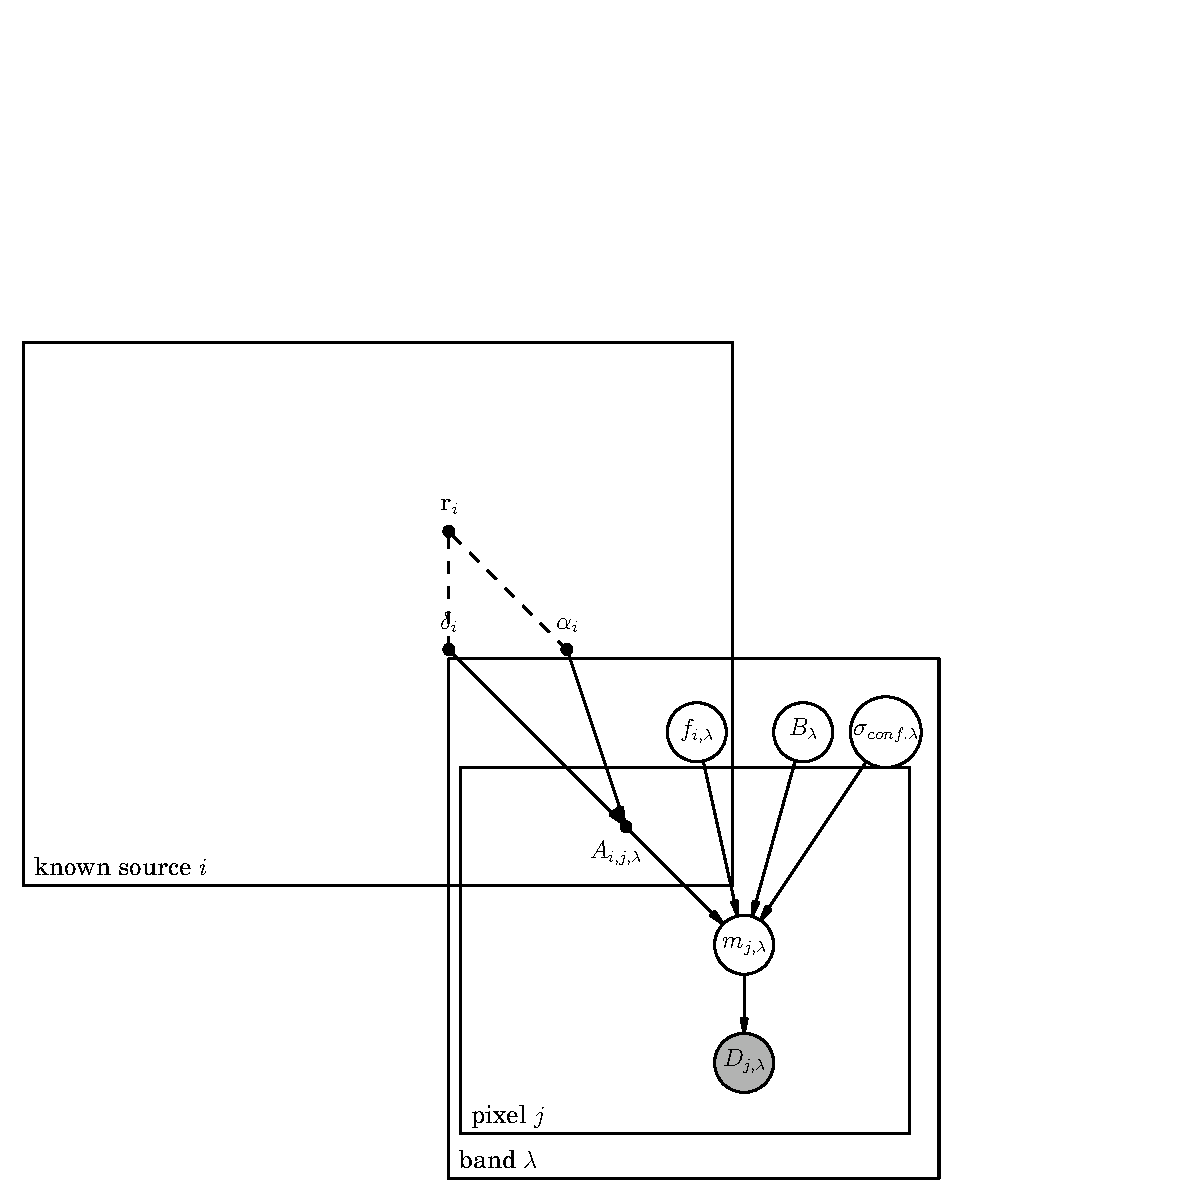
\includegraphics[width=8.5cm]{./graphical_model.pdf}
\caption{Our probabilistic model for XID+. Boxes represent dimensions, open circles as variables, dots as deterministic or (fixed) variables. Created with DAFT (\url{http://daft-pgm.org/})}\label{fig:graph_mod_xid+}
\end{figure}
 
\subsubsection{Stan}
Now we have our probabilistic model, we need a Bayesian inference tool capable of sampling from it to obtain the posterior. We use the Bayesian inference tool, \textit{Stan}, which is `a probabilistic programming language implementing full Bayesian statistical inference with MCMC sampling'. \textit{Stan} uses the adaptive Hamiltonian Monte Carlo (HMC) No-U-Turn Sampler (NUTS) of Hoffman & Gelman (In press) to efficiently sample from the posterior. It does this by using the gradient, which allows fast traversing of high dimensional and highly correlated joint posterior distributions. 

\textit{Stan} has its own modelling language, in which one constructs probabilistic models. Our model for \textit{Stan} can be found in Appendix A.
\subsubsection{Estimating Convergence}
As with all MCMC routines, one needs to run enough chains and run them long enough to be confident the global minimum has been found and that it has been thoroughly sampled. 

As default, we run four separate chains from different initial positions. We also discard the first half of the chain as `warm up' to ensure the chains have converged to the posterior distribution. We then assess the convergence of each parameter by comparing the variation between and within chains using the diagnostics described in \cite{BDA3} which can be summarised as follows: Each chain is split in two and the between ($B$) and within chain ($W$) variance is calculated. $B$ and $W$ are then used to calculate the marginal posterior variance. This in turn can be used to estimate the potential scale reduction $\hat{R}$, which reduces to 1 as the number of iterations tends to infinity. An $\hat{R}$ value $\gt 1.2$ suggests chains require more samples. We provide $\hat{R}$ for each parameter.

Due to the nature of MCMC, samples from MCMC routines are correlated. Inference from correlated samples is less precise than from the same number of independent draws. In order to check there are enough independent draws we estimate the effective number of samples $\hat{n_{eff}}$, defined in \cite{BDA3}. We require $\hat{n_{eff}}$ to be 10 times the number of chains and provide the estimate for each parameter.

\subsection{Map segmentation}
The survey fields in HELP vary in size from .... to ..... square degrees. Ideally, source photometry and background estimation would be done on the full image, in practice it is often computationally infeasible. DESPHOT segmented the map by locating islands of high SNR pixels enclosed by low SNR pixels. The segmentation algorithm operates thus:
\begin{itemize}
\item Locates all pixels with a SNR above some threshold (default value of SNR= 1);
\item Takes the first of these high SNR pixel starting in the bottom left corner of the image;
\item `Grows' a region around this pixel by iteratively taking neighbouring high SNR pixels;
\item Once there are no more high SNR neighbours jumps to the next high SNR pixel and repeat from step (iii).
Each of these independent regions of high SNR pixels is uniquely identified and processed separately by the source photometry component.
\end{itemize}

For XID+, we first investigated using the most optimum and transparent way of segmenting the map. This involves breaking the map into distinct tiles but fitting for sources within and beyond the tiling region. Using the fact that, conditional on the fluxes, the data from each tile is independent, the posterior from the different tiles can be combined to give an overall posterior for the whole map using the following formula:

\begin{equation}
P(\mathbf{F}|D_1,..D_n,D_A)=a\frac{\prod_{i=1}^n P(\mathbf{F}|D_n,D_A)}{P(\mathbf{F}|D_A)^{n-1}}
\end{equation}

where $n$ is number of tiles and $P(\mathbf{F}|D_A)$ is our prior on the flux, given some ancillary data. As the number of dimensions is highly dimensional, the only feasible way of multiplying highly dimensional probability distribution functions is to model them as multivariate Gaussians. We investigated fitting the fluxes in both normal and log space in an attempt to make the multivariate Gaussian approximation appropriate. Unfortunately, neither succeeded and so we have to abandon the optimum scheme.

We have settled on a tiling scheme that has tiles that overlap in the map. This makes sure sources that lie near the edge of a tile, will be nearer the centre of the adjacent tile. As before, for each tile, we fit to sources both in and beyond. For our final posterior, for each source, we take the posterior form the tile that is optimum, i.e. the tile in which the source lies closest to the centre.

\subsection{Uncertainties and Covariances}
If DESPHOT is assumed to be linear\footnote{introducing LASSO and non-negative priors introduces a non-linearity}, then one can get a lower limit on the noise from $(\mathbf{A^TN_d^{-1}A})^{-1}$. This estimate only includes instrumental noise and degeneracies between sources. An estimate of the remaining residual confusion noise is is calculated by taking the standard deviation of the residual map pixels $\sigma{res}$ and removing the average instrumental noise in these pixels in quadrature, $\sigma^2_{conf} = \sigma^2_{res} - \sigma^2_{pix}$, where $\sigma_{pix}$ is calculated directly from the exposure time per pixel. The total noise $\sigma_{tot}$ for a point source is then calculated from both the instrumental noise (and confusion noise from the known sources), $\sigma_{i} = \sqrt{\mathrm{diag}((\mathbf{A^TN^{-1}_dA)^{-1})}}$, and confusion noise from the unknown sources in the residual map $\sigma_{conf}$ via $\sigma^2_{tot} = \sigma^2_{i} + \sigma^2_{conf}$. 

%Details on what we get out of fit. e.g. marginalised estimate of fluxes, covariance information between sources
For XID+ we are sampling directly from the posterior which give the uncertainty of the flux given the data. This includes the uncertainty from instrumental noise and confusion (I think). Unlike XID, we are not solving $\mathbf{f}=(\mathbf{A^TN_d^{-1}A})^{-1}\mathbf{A^TN_d^{-1}d}$, we are solving equation \ref{eq:map} and so variations in pixel flux from sources not in the prior list, i.e. from confusion, will directly affect our flux estimates. This is advantageous as DESPHOT was well known to underestimate the uncertainties.


\section{Simulations}
In order to test and quantify XID+, we use simulated SPIRE maps, generated from the Lacey simulations. NEED MORE DETAIL

A mock 100 $\mathrm{\mu m}$ input catalogue, similar to that expected from a PACS catalogue, is generated by taking the mock catalogue and making a cut at a flux limit of 50 $\mathrm{mJy}$. We use this as our prior input catalogue for both XID+ and DESPHOT. In order to compare performance, we look at three measures: precision, flux accuracy, and flux error density.

\subsection{Flux Precision}
Precision is a measure of how well the flux is believed to be constrained. Figures \ref{} and \ref{} show how the precision of XID+ and DESPHOT change as a function of input flux for a deep (confusion noise dominated) and shallow (instrumental noise dominated ) simulation, for all three bands. 

\subsection{Flux Accuracy}
Flux accuracy is a measure of how far away the estimated flux is from the truth.


\subsection{Flux Error density}
Flux error density measures how well the estimated uncertainty is correct. For well estimated errors, the distribution of $S_{in} - S_{out}$ should be centred on zero, and for 68.27\% of the time, lie within one sigma, while 95.45\% lie within 2 sigma. Figure \ref{} shows the flux error density as a function of input flux. 

flux accuracy (i.e. $S_{obs} - S_{True}$), measured across all recovered sources. Figure \ref{Fig:flux_acc} shows the flux accuracy for both XID+ and DESPHOT while Table \ref{} shows the mean flux accuracy for both methods.

\begin{figure}
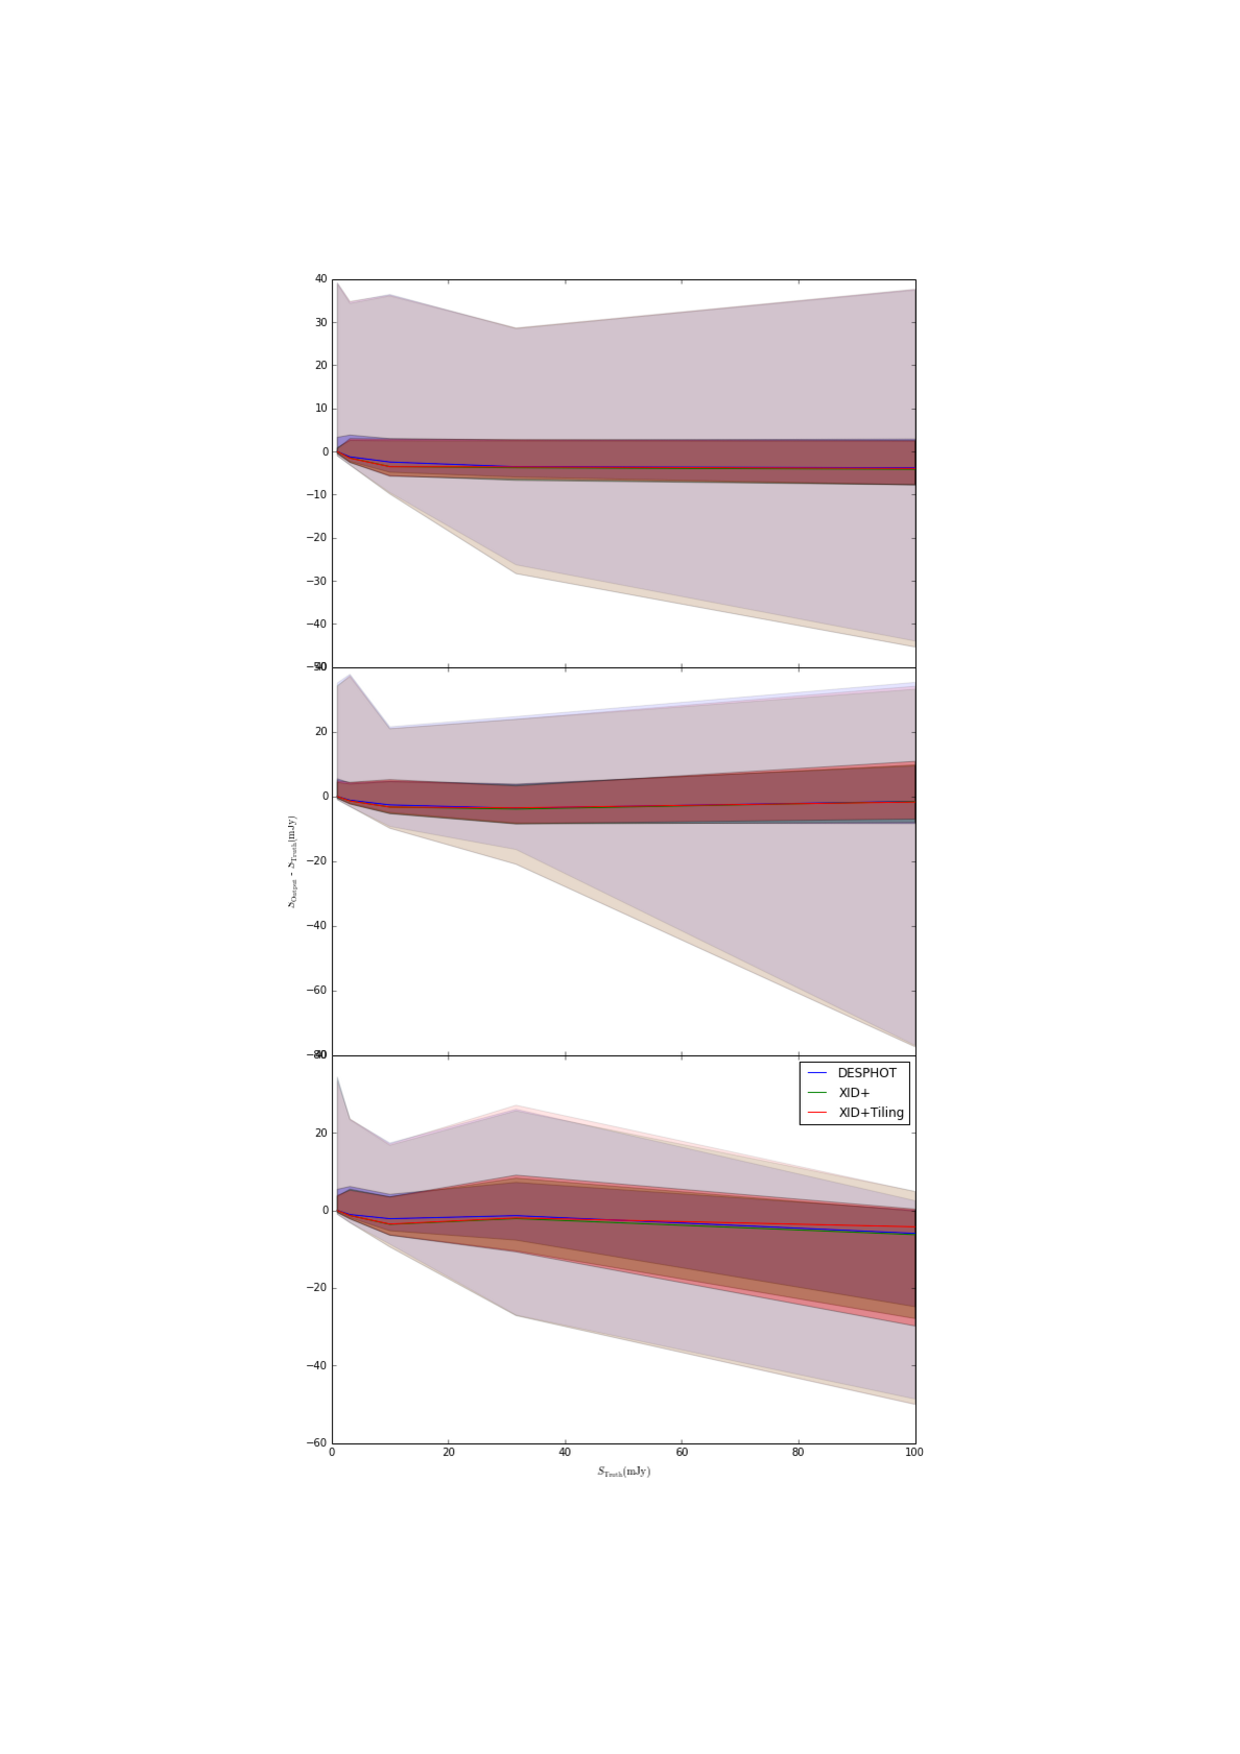
\includegraphics[width=8cm]{./Figures/Flux_accuracy}
\caption{The Flux accuracy for DESPHOT, XID+ and XID+Tiling for the three SPIRE bands. The lines indicate median flux accuracy, the darker filled regions indicate the one sigma dispersion limit, while lighter filled regions indicate the three sigma limit of dispersion.}\label{Fig:flux_acc}
\end{figure}

It is also vital that our proposed method return reliable estimates of the flux density error, as for real applications we will not have knowledge of the true flux density of our sources. In Figure \ref{Fig:flux_density_error} we show the distribution of observed flux density error (i.e. $S_{obs}-S_{true}$), normalised by the error estimated by the photometric pipeline for the deep simulation. 

\begin{figure}
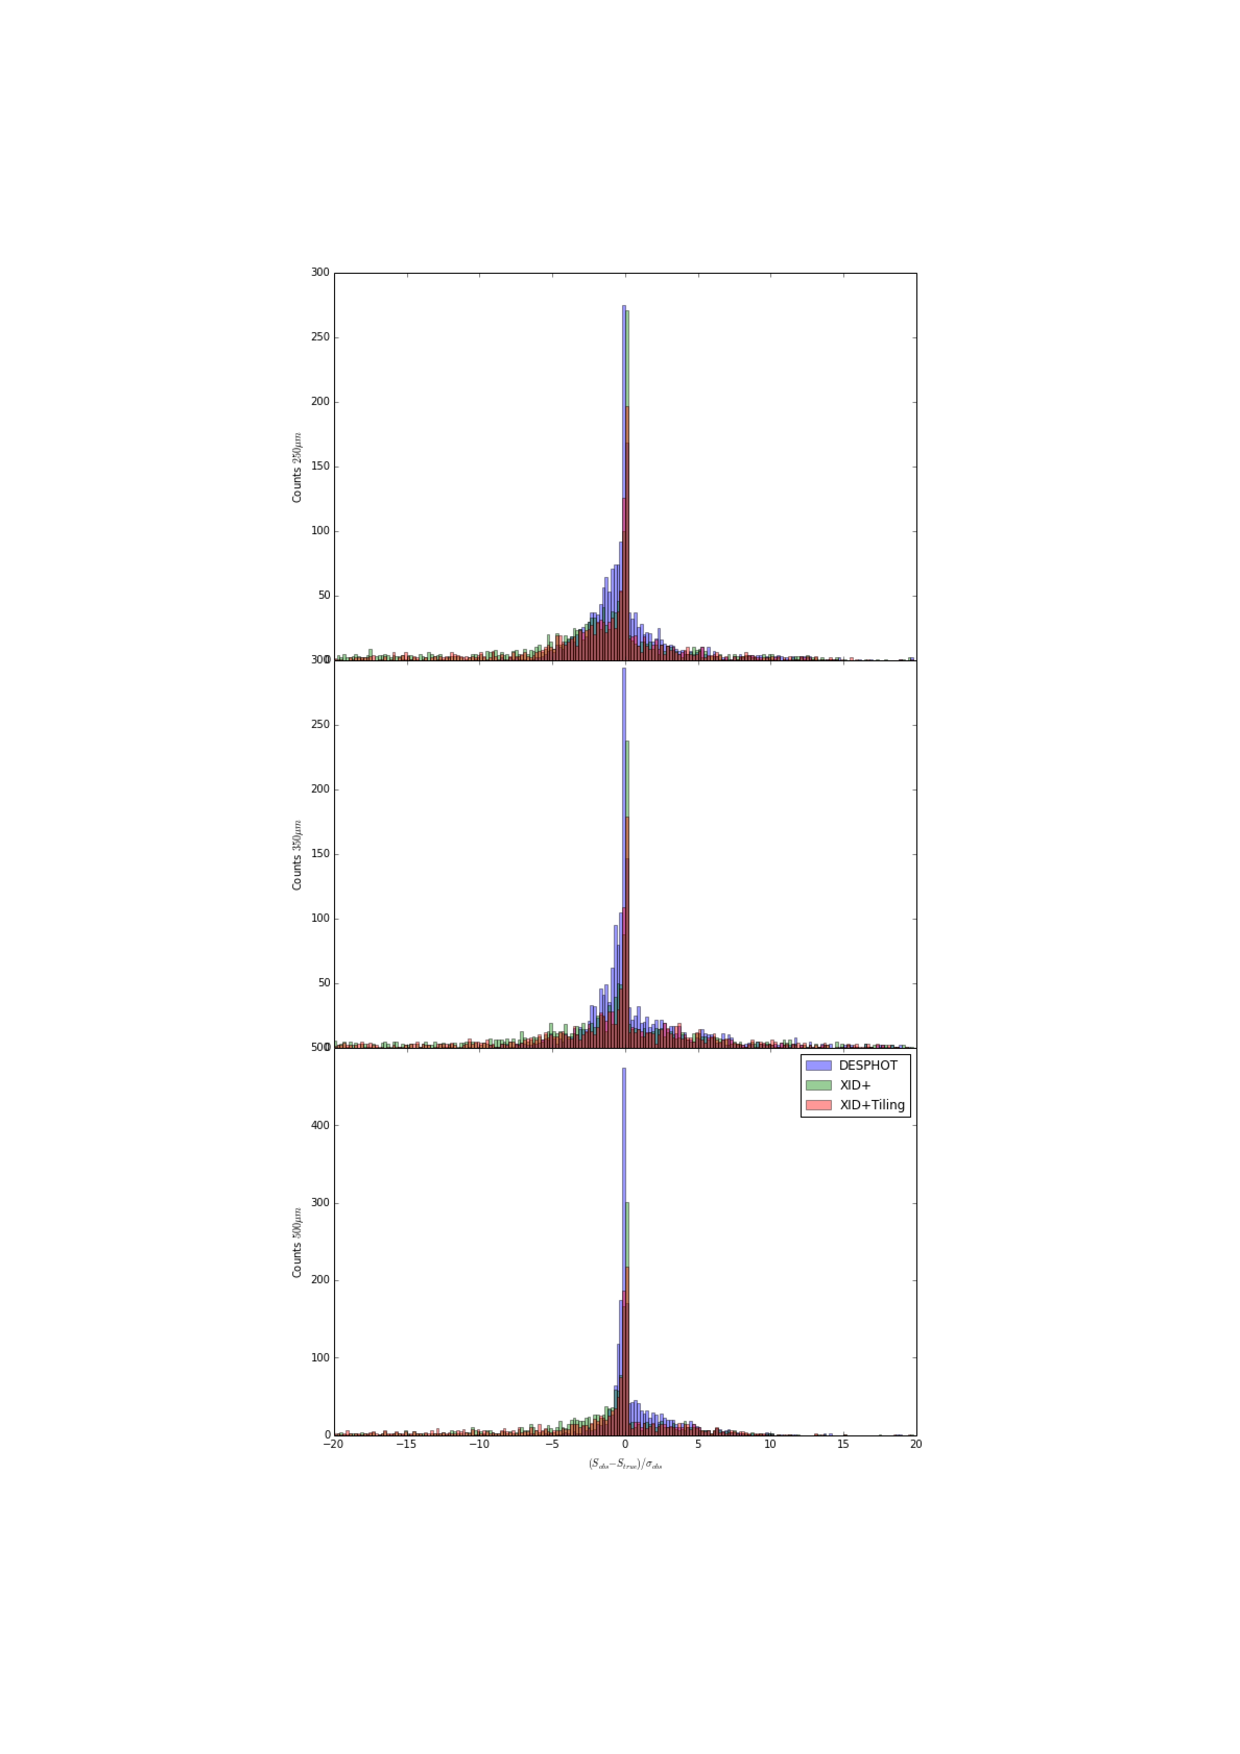
\includegraphics[width=8cm]{./Figures/Flux_density_error}
\caption{The Flux density error for DESPHOT, XID+ and XID+Tiling for the three SPIRE bands.}\label{Fig:flux_density_error}
\end{figure}

\subsection{Correlated Sources}
For sources that lie close together, the uncertainty on the flux estimates is correlated between the sources. One of the advantages of obtaining the full posterior is we get a proper estimate of uncertainty and its correlation. This is particularly apparent when comparing with DESPHOT, which, by using the LASSO algorithm would force one source to have all the flux and the other nearby source to zero. Figure \ref{} shows an example of two nearby sources. The posterior provided by XID+, fully captures the correlated uncertainty, where as the `winner takes all' approach from DESPHOT clearly fails to estimate the true flux for both sources.

\subsection{Real data}
% inject sources into map and recover




\section{XID+Science}
%Show how framework allows users to do science with maps 
%Posterior predictive checks comes in showing model is correct. This should really come when pushing model to do science
\subsection{Stacking}
Traditional stacking has been used on the Herschel maps to find fluxes for groups of objects. The traditional approach finds the mean flux.

With XID+, we can use a hierarchical structure to properly model the flux distribution sources wishing to be stacked. In principle, we can model what stacking does. 

Other thoughts.. by having only one background, sources that are faint are not being modelled properly as they could sit under background level.
\section{Conclusions}



\section*{Acknowledgements} %
%
%%
%
%
\bibliography{}
\appendix
\section*{Appendix A}\label{Stan_model}
\onecolumn
\lstinputlisting[language=C, linewidth=18cm]{../stan_models/XID+SPIRE.stan}
%
%
%
%
%
%%%%%%%%%%%%%%%%%%%%%%%%%%%%%%%%%%%%%
%
%% \bsp % ``This paper has been produced using the ...''
%
%\label{lastpage}

\end{document}
